\begin{figure}[h!]
    \begin{center}
    \caption{Effects on Primary Care Coverage - Intensive Margin}\label{fig:9}
    \begin{subfigure}{0.32\textwidth}
        \caption{\scriptsize N. of People Visited}\label{fig:9a}
        \centering
        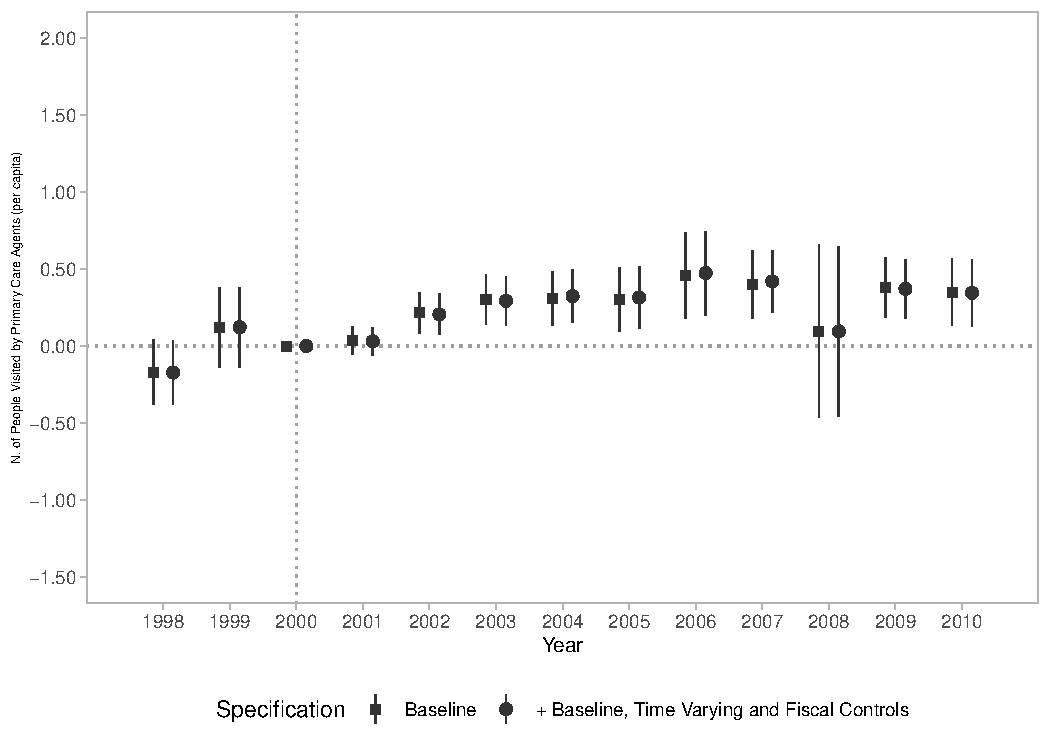
\includegraphics[width=\textwidth]{plots/siab_accomp_especif_pcapita_dist_ec29_baseline_dist_ec29_baseline_9.pdf}
    \end{subfigure}
    \begin{subfigure}{0.32\textwidth}
        \centering
        \caption{\scriptsize People Visited by CH Agents}\label{fig:9b}
        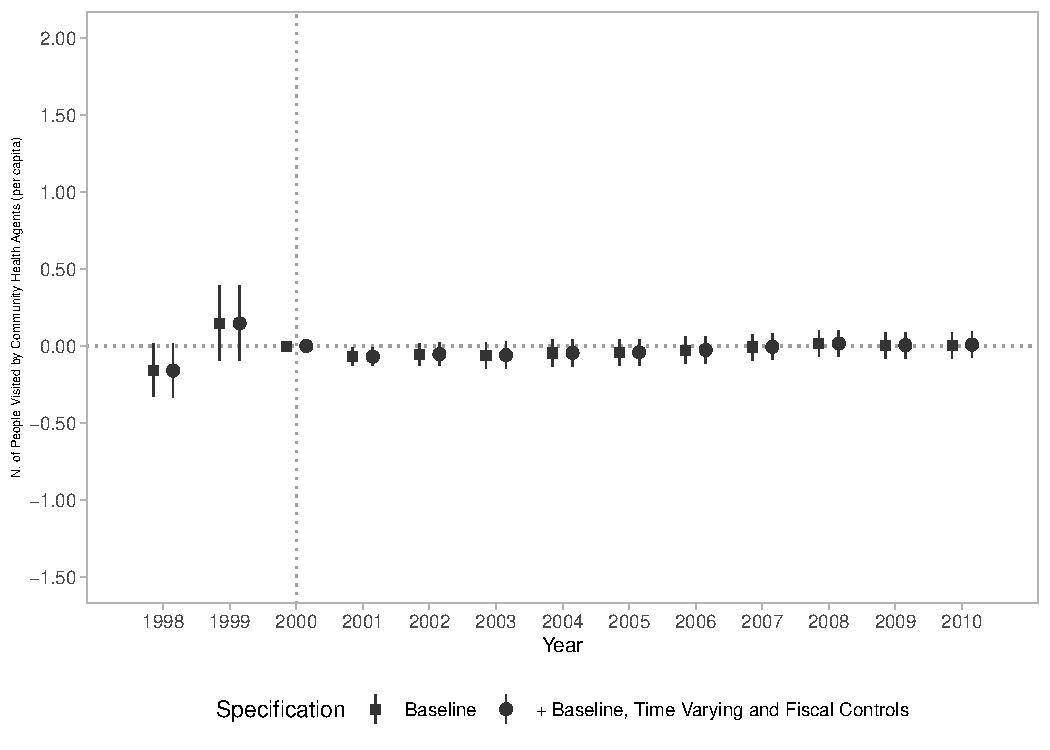
\includegraphics[width=\textwidth]{plots/siab_accomp_especif_pacs_pcapita_dist_ec29_baseline_dist_ec29_baseline_9.pdf}
    \end{subfigure}
    \begin{subfigure}{0.32\textwidth}
        \centering
        \caption{\scriptsize People Visited by FH Agents}\label{fig:9c}
        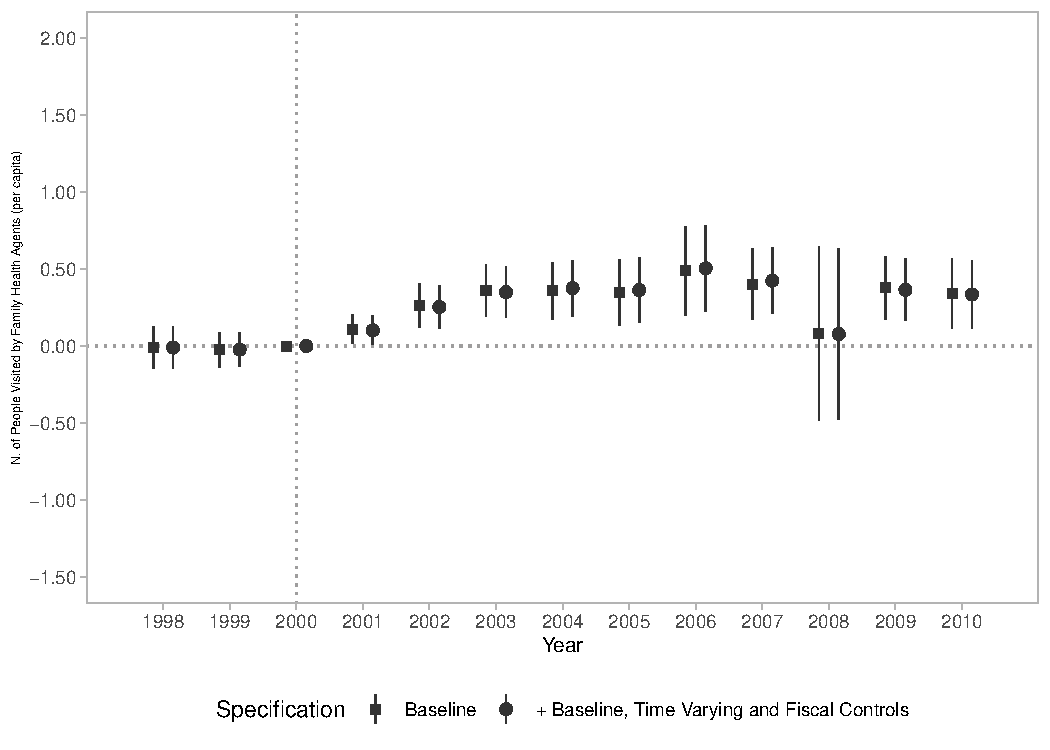
\includegraphics[width=\textwidth]{plots/siab_accomp_especif_psf_pcapita_dist_ec29_baseline_dist_ec29_baseline_9.pdf}
    \end{subfigure}
        \begin{subfigure}{0.32\textwidth}
        \caption{\scriptsize N. of Household Visits and Appointments}\label{fig:9d}
        \centering
        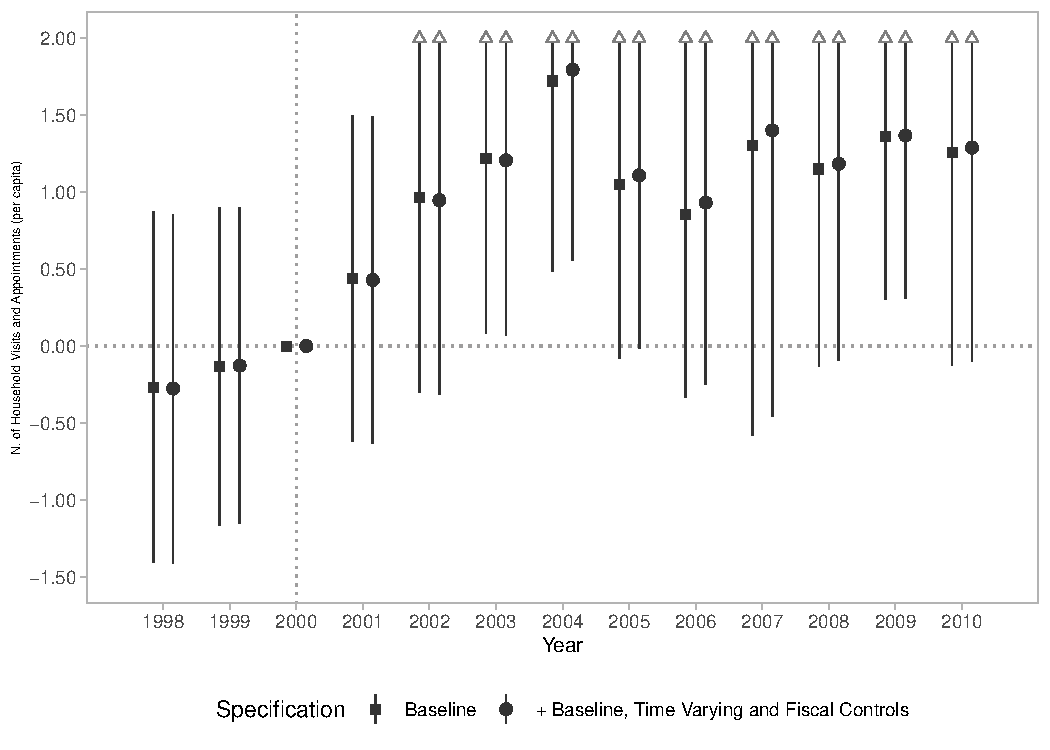
\includegraphics[width=\textwidth]{plots/siab_visit_cons_pcapita_dist_ec29_baseline_dist_ec29_baseline_9.pdf}
    \end{subfigure}
    \begin{subfigure}{0.32\textwidth}
        \centering
        \caption{\scriptsize N. of Household Visits and Appointments by CH Agents}\label{fig:9e}
        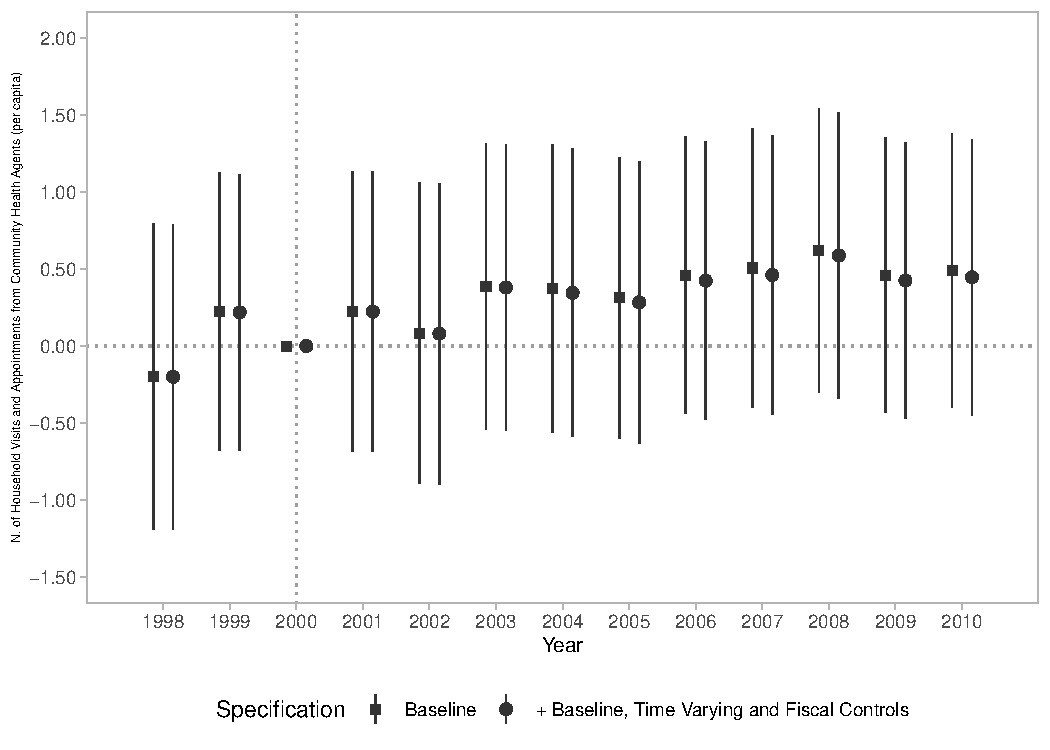
\includegraphics[width=\textwidth]{plots/siab_visit_cons_pacs_pcapita_dist_ec29_baseline_dist_ec29_baseline_9.pdf}
    \end{subfigure}
    \begin{subfigure}{0.32\textwidth}
        \centering
        \caption{\scriptsize N. of Household Visits and Appointments by FH Agents}\label{fig:9f}
        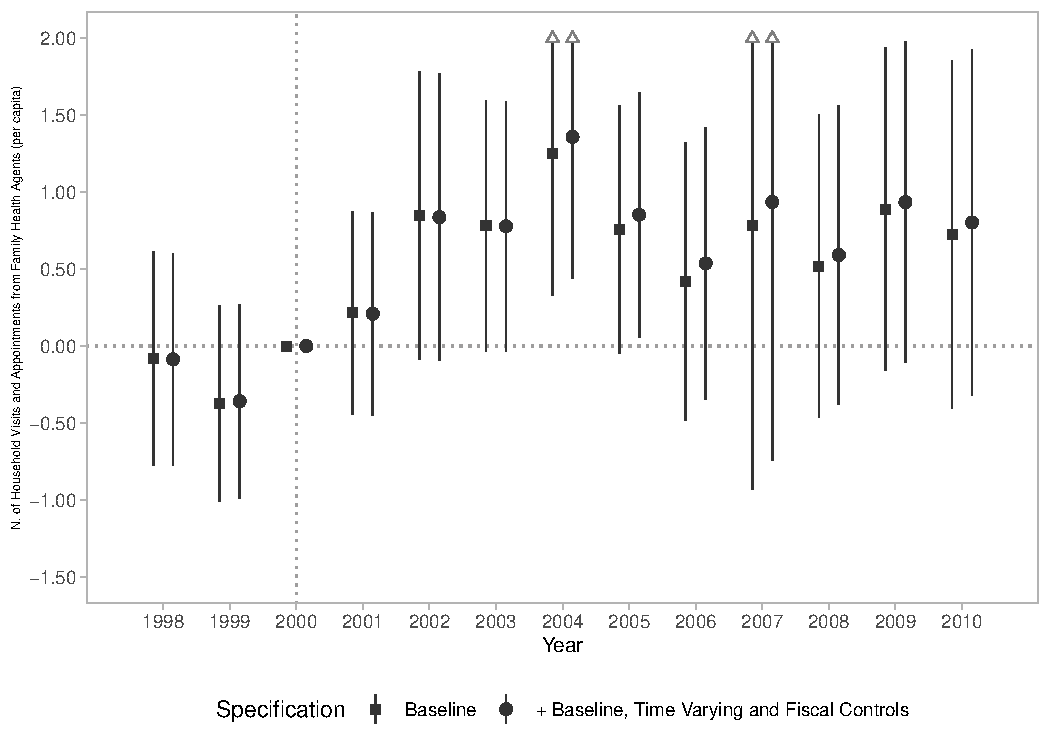
\includegraphics[width=\textwidth]{plots/siab_visit_cons_psf_pcapita_dist_ec29_baseline_dist_ec29_baseline_9.pdf}
    \end{subfigure}
    
    \end{center}
    
            \scriptsize{Notes: The number of observations is 64482. DiD Estimates from Equation \ref{eq:2}. Independent variable is the distance to the EC/29 target in p.p. Square dots represent the baseline model with municipality and state-year fixed effects. Round dots represent fully saturated specification (Column 4 in regression Tables). Lines represent 95\% confidence intervals. Arrows, when present, indicate confidence intervals out of the plot bounds. Standard errors are clustered in the municipality level.}
    
\end{figure}